\setchapterpreamble[u]{\margintoc}
\chapter{Crittografia in cascata}
\labch{chapter2}

L'idea è di provare a mettere in cascata una serie di sistemi crittografici deboli (es: usando chiavi piccole) per vedere se si riescono a ottenere sistemi più forti. 

\section{Permutazioni in cascata} 
Ho un rullo a due facce. Su ciascuna faccia sono presenti 26 contatti, che rappresentano le 26 lettere dell'alfabeto. Un qualsiasi collegamento interno al cilindro tra le due facce mi rappresenta una possibile permutazione (es: sul lato del plaintext premo il contatto che rappresenta la A e ottengo sull'altro lato, che mi rappresenta il cyphertext la lettera P). Suppongo di scegliere per il rullo la permutazione $\Pi_1$. Collego ora alla faccia del cyphertext del rullo un secondo rullo (che funziona esattamente come il primo) e per lui scelgo la permutazione $\Pi_2$. Aggiungo un terzo rullo collegato alla faccia cyphertext del secondo e scelgo la permutazione $\Pi_3$. Il mio sistema è diventato più resistente? No. La combinazione delle 3 (o anche $n$) permutazioni $\Pi_1 \circ \Pi_2 \circ \Pi_3$ è, alla fine, una permutazione, che sarà identica per ogni lettera del testo che voglio cifrare.
Provo quindi a creare una soluzione più robusta. Decido ora di ruotare il terzo cilindro di una posizione dopo aver codificato ogni lettera del plaintext. Con questa soluzione non ho più una permutazione unica associata all'intero plaintext, ma una per ogni sua lettera, fino ad un massimo di 26 shift, in quanto poi ritorno alla posizione iniziale. Ovviamente, se decido di ruotare il secondo rullo per ogni giro completo, incremento il numero di permutazioni uniche che posso usare ($26^2$).

\section{Enigma} 
Enigma usava un metodo di cifratura molto simile a quello descritto sopra. La sua vulnerabilità non stava tanto nel sistema, ma nel fatto che ogni messaggio scambiato iniziava sempre con lo stesso testo, dal quale gli attaccanti sono riusciti a romperla. Enigma era quindi vulnerabile al \textbf{known plaintext attack}.

\section{Tipi di attacchi} 
Vediamo gli attacchi che un sistema crittografico può affrontare per essere considerato affidabile:
\begin{itemize}
    \item Known cyphertext attack: l'attaccante conosce solo il testo cifrato del messaggio;
    \item Known plaintext attack: l'attaccante conosce il messaggio in chiaro e il relativo cyphertext;
    \item Chosen plaintext attack: l'attaccante sceglie il messaggio da cifrare e analizza il relativo cyphertext;
    \item Adaptive chosen plaintext attack: l'attaccante sceglie il testo di un primo messaggio, analizza il cyphertext ottenuto e in base all'analisi sceglie un nuovo messaggio da cifrare e così via.
\end{itemize}

Se, ad esempio, il sistema è vulnerabile ad un \textit{adaptive chosen plaintext attack}, sarà più affidabile di un sistema che è debole ad un \textit{known cyphertext attack}.

\section{Nascita di DES} 
Col tempo diventa necessario avere un sistema crittografico standard internazionale. Tra le proposte alla fine ne venne scelta una e il protocollo venne chiamata Data Encryption Standard (DES). DES venne costruito con l'idea di durare una ventina d'anni, come è effettivamente stato. DES venne bucato con la \textbf{crittoanalisi differenziale}.

A partire da due input \textit{x} e \textit{y} e i rispettivi cyphertext \textit{E(x, k)} e \textit{E(y, k)} cifrato con chiave \textit{k}, questa analisi confrontava lo XOR degli input con lo XOR dei cyphertext. Praticamente analizzava come le differenze tra i bit di ingresso si propagassero nei bit di uscita. 

\begin{center}
    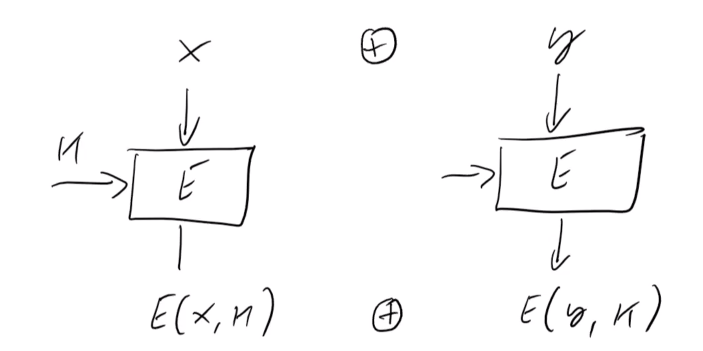
\includegraphics[width=1\textwidth]{images/1.png}
\end{center}

\noindent L'analisi ritornava un'equazione lineare sui bit della chiave \textit{k}, permettendo di costruire alla fine un sistema di equazioni indipendenti a 56 variabili, che rappresentano i 56 bit della chiave usata da DES. Si è scoperto che fissando 12 variabili, era possibile risolvere il sistema, e quindi ottenere la chiave. Di conseguenza, un attaccante non doveva più ricavare 56 bit, ma solo 12 (in quanto gli altri 44 sono ricavabili da questi), riducendo il numero di tentativi necessari per un attacco a forza bruta a solo $2^{12} = 4096$ tentativi.

\noindent Per fare questa analisi è necessario utilizzare un \textit{adaptive chosen plaintext attack}.

\section{Nascita di AES} 
Scoperta la debolezza di DES, si cercarono nuovi protocolli per sostituirlo, che fossero resistenti alle sue vulnerabilità. Venne scelto l'algoritmo che poi venne chiamato Advanced Encryption Standard (AES), che è quello usato oggi. Sostanzialmente è una sequenza di quattro fasi, ognuna delle quali va a contrastare uno degli attacchi noti a DES. Sia per DES che per AES, non esiste una vera e propria dimostrazione che il sistema sia robusto, ma c'è solamente una analisi che dice "ci abbiamo provato in tanti e abbiamo una ragionevole convinzione che saranno robusti almeno per un po' di tempo". 

\paragraph{Fattorizzazione di un numero} In generale, non esiste un modo per costruire un protocollo dove si sa che sia sicuro alla base, ovvero che sappiamo che invulnerabile ad attacchi presenti e futuri, eccetto per one-time pad, dove abbiamo visto che esiste una dimostrazione che funzione ed è sicuro. 

Gli algoritmi attualmente esistenti di fattorizzazione di un numero provano tutti i possibili divisori del numero, ed hanno una complessità esponenziale al numero di bit del numero. Molte persone, appartenenti ad abiti diversi, hanno provato a trovare un algoritmo più ottimizzato, ma senza successo. Verosimilmente un algoritmo efficiente per fattorizzare un numero non verrà trovato. Quindi, se si riuscisse a costruire un crittosistema per il quale è possibile dire che se si trova un algoritmo per attaccarlo allora si è trovato un algoritmo per fattorizzare un numero, allora in questo caso si può dire che l'attaccante non ci possa riuscire. 

\section{Overview di DES}

\begin{center}
    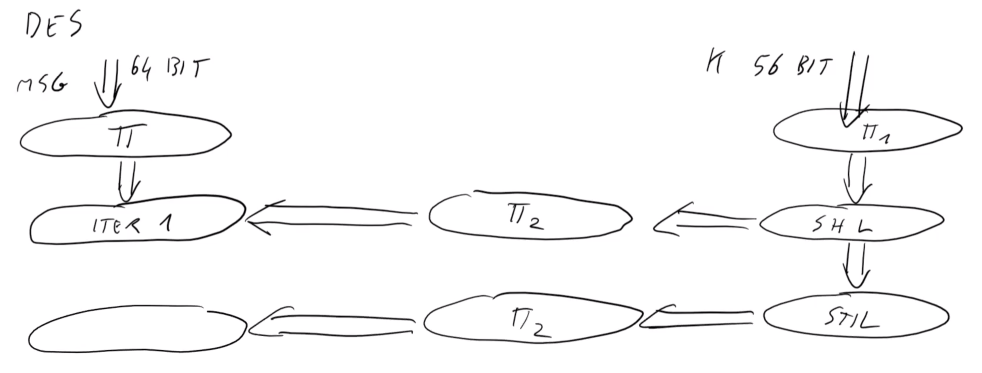
\includegraphics[width=1\textwidth]{images/2.png}
\end{center}

Dato un messaggio di 64 bit e una chiave di 56 bit, DES prevede i seguenti passi:

\begin{enumerate}
    \item Permuto con permutazione $\Pi$ il messaggio;
    \item Permuto la chiave \textit{k} con permutazione $\Pi_1$;
    \item Shifto con rotazione la chiave permutata a sinistra di una posizione;
    \item Applico la permutazione $\Pi_2$ alla chiave shiftata;
    \item Applico la chiave ottenuta al messaggio permutato, utilizzando il meccanismo di \textbf{Feistel};
    \item Ripeto i passi 3, 4 e 5 per 16 volte;
    \item Applico infine al risultato $\Pi^{-1}$, ovvero calcolo ,a permutazione inversa a quella iniziale.
\end{enumerate}

\noindent Le permutazioni usate non aggiungono nulla dal punto di vista della sicurezza del sistema, riguardano infatti l'aspetto fisico del sistema: poiché il sistema è implementato in un chip non è detto, per ragioni di ottimizzazione dello spazio, che contatti di entrata e di uscita si trovino nello stesso ordine.
\\

\noindent Il meccanismo di Feistel è fatto in modo che l'algoritmo di codifica e decodifica siano uguali. Questa soluzione mi costa meno a livello di hardware, in quanto mi basta un solo chip. Le chiavi però devono essere usate, nella decodifica, in ordine inverso rispetto alla codifica. Lo scopo di Feistel era quello di creare uno schema dove algoritmo di codifica e decodifica fossero gli stessi e che fosse applicabile a crittosistemi diversi.

\begin{center}
    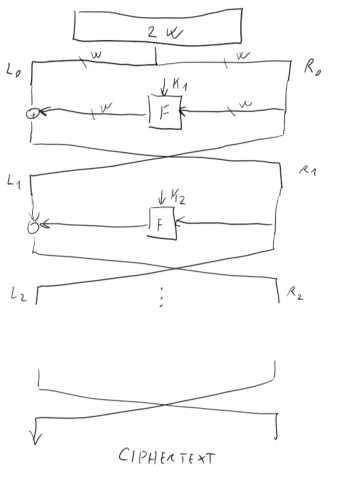
\includegraphics[width=1\textwidth]{images/3.png}
\end{center}

Lo schema di Feistel prende in input un flusso di dati in ingresso di dimensione $2W$ (con $W$ numero arbitrario) ed esegue le seguenti operazioni:
\begin{enumerate}
    \item Divide il messaggio iniziale in due messaggi $L_0$ e $R_0$ entrambi di dimensione $W$;
    \item $R_0$ viene applicato ad una funzione qualsiasi $F$, con chiave $k_1$, e produce un nuove messaggio di dimensione sempre $W$;
    \item Il messaggio risultate al punto 2 viene messo in XOR col messaggio $L_0$;
    \item Il messaggio $R_0$ e il messaggio risultatane dal punto 3 vengono scambiati di posizione, diventando il messaggio $L_1$ e $R_1$;
    \item I punti 2, 3 e 4 vengono ripetuti per $n$ volte, utilizzando sempre una chiave diversa ($k_2$, $k_3$, ...);
    \item Eseguo un ultimo scambio tra il messaggio di destra e quello di sinistra, ottenendo il cyphertext.
\end{enumerate}

\noindent La caratteristica interessante di questo schema è che indipendentemente dalla funzione $F$ l'applicazione di questo protocollo a partire dal cyphertext con le chiavi in ordine inverso produce il plaintext. Quindi $F$ può essere qualsiasi funzione. 
\\

\noindent Supponiamo ora di avere il seguente schema di Feistel dicodifica e decodifica, con quattro passi, dove non scambio i due lati, ma ci cambio solo il nome, eccetto per il passo finale.\\

\begin{center}
    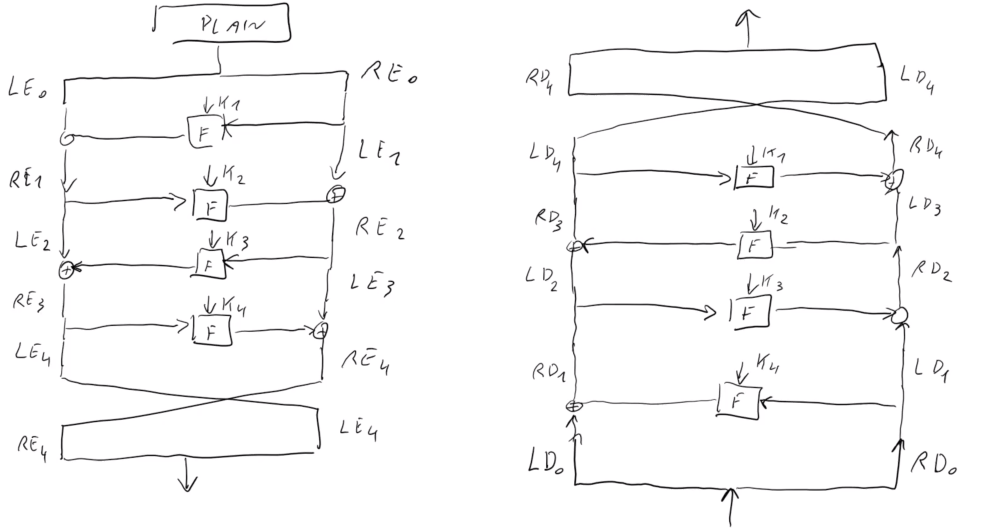
\includegraphics[width=1\textwidth]{images/4.png}
\end{center}

\noindent Dimostriamo ora che i due schemi sono identici:
\begin{align*}
    LD_1 = RD_0 = LE_4 = RE_3\\
    RD_1 = LD_0 \oplus F(K_4, RD_0) &= RE_4 \oplus F(K_4, RE_3)\\
                                    &= LE_3 \oplus F(K_4, RE_3) \oplus F(K_4, RE_3)\\
                                    &= LE_3
\end{align*}      

\noindent Quindi la \textit{Left Decryption 1} equivale alla \textit{Right Encryption 3} e la \textit{Right Decryption 1} equivale alla \textit{Left Encryption 3}. Questa dimostrazione può essere estesa anche ai restanti tre passi, andando a confermare che lo schema di Feistel per codifica e decodifica è lo stesso. 

Come si può vedere, la funzione \textit{F} va solo ad aggiungere confusione; il prodotto del plaintext per la funzione viene automaticamente rimosso durante la decodifica, a prescindere da cosa sia. La \textit{F} ha il compito di rendere difficile la decodifica non conoscendo quale sia la chiave. 

\begin{center}
    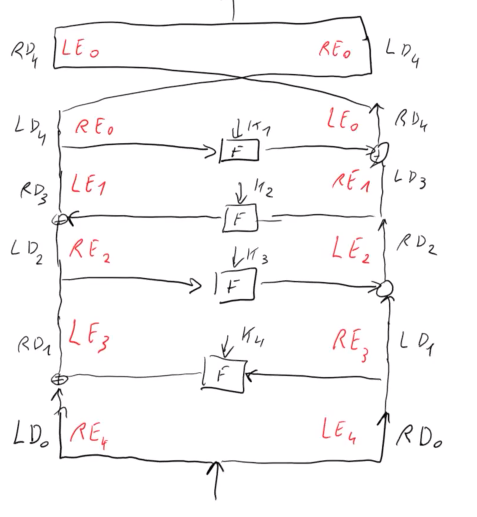
\includegraphics[width=1\textwidth]{images/5.png}
\end{center}
